\documentclass{article}

\usepackage[a4paper,left=18mm,right=18mm,top=20mm,bottom=18mm]{geometry}
\usepackage[italian]{babel}

\usepackage{titling}
\usepackage{graphicx}
\usepackage{subcaption}
\usepackage{float}

\title{Report analisi dell'aria}
\author{David Guzman Piedrahita e Marco Vinciguerra}
\date{\today}

\makeatletter         
\def\@maketitle{
\noindent\begin{minipage}{\textwidth}
\begin{minipage}[c]{0.8\textwidth}  
\begin{center}
{\Huge \bfseries \sffamily \@title }\\[4ex] 
{\Large  \@author}\\[4ex] 
\@date\\[0ex]
\end{center}
\end{minipage}\hfill
\begin{minipage}[c]{0.2\textwidth}
\raggedleft

\includegraphics[width = 20mm]{Picture/logo.png}\\[0.1ex]

\includegraphics[width = 25mm]{Picture/UniBg-logo.jpg}
\end{minipage}
\end{minipage}  
}
\makeatother


\begin{document}

\maketitle

\par\noindent\rule{\textwidth}{0.4pt}
\textbf{Abstract:} Paper preliminare per la tesi di laurea (gestione dei dati inquinanti-meteo)
\par\noindent\rule{\textwidth}{0.4pt}

\section{Introduzione}
La fase iniziale del progetto consiste nell'analisi nell'arco temporale 2018-2020 dei dati 
forniti dal sito ARPAL relativi allo studio del $NH_{3}$ e dei particolati atmosferici $PM10$ e $PM2.5$ al 
fine di dimostrare una possibile correlazione tra di essi. 
E' stato scelto questo periodo di tempo perchè ci si aspetta che i dati continuino a essere rilevati nel futuro
e si auspica che riflettano i comportamenti più recenti di questi inquinanti in un modo più accurato.
\\Ogni stazione misura diversi inqunanti a seconda dei sensori installati e/o può anche misurare anche dati meteo.
Le mappe della delle stazioni che rilevano gli inquinanti e meteo sono le 
seguenti:
\begin{figure}[h!]         
    \centering
    \begin{subfigure}{.5\textwidth}
      \centering
      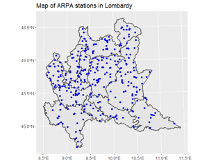
\includegraphics[width=.7\linewidth]{Picture/Lpollution.png}
      \caption{Stazioni meteo}
      \label{fig:sub1}
    \end{subfigure}%
    \begin{subfigure}{.5\textwidth}
      \centering
      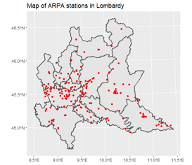
\includegraphics[width=.7\linewidth]{Picture/Lweather.png}
      \caption{Stazioni inquinanti}
      \label{fig:sub2}
    \end{subfigure}
    \label{fig:test}
\end{figure}
\\Come si può osservare, entrambe le reti di centraline non sono equidistanti tra loro e non formano 
una rete omogenea. La corrispondenza non univoca dovrà quindi essere gestita.

\section{Analisi preliminare dei dati per gli inquinanti}
La fase iniziale del progetto consiste nel cercare le centraline in Lombardia
che misurano contemporaneamente $NH_{3}$, $PM10$ e $PM2.5$ oppure solo due di essi
, in quanto non è possibile
studiare le relazioni tra questi inquinanti se solo uno dei tre è disponibile.
Sono comunque ammessi dei dati mancanti sporadicamente.
\\E' importante anche tenere conto della frequenza con cui i dati non vengono misurati, visto che questo
fattore può determinare se un dataset è rappresentativo del vero comportamento degli inquinati nel mondo reale.
\\In totale ARPA Lombardia mette a disposizione 174 stazioni di qualità dell'aria e 279 stazioni 
meteorologiche.
Le centraline che misurano tutti e 3 gli inquinanti sono solamente 6 e sono le seguenti:
\begin{itemize}
    \item Cremona via Fatebenefratelli (ID station: 677)
    \item Schivenoglia (ID station: 703)
    \item Sannazzaro de Burgondi Agip (ID station: 693)
    \item Pavia via Folperti (ID station: 642)
    \item Milano Pascal Citta Studi (ID station: 705)
    \item Moggio (ID station: 681)
\end{itemize}
Bisogna sottolineare che tutti i risultati finora ottenuti riguardano il 2018, ma, ripetendo le stesse analisi per il 2019 e il 2020, 
le centraline che rilevano tutte e tre le variabili risultano essere le stesse 6.
Le stazioni che ne misurano solo due regressori di interesse sono in totale 26.
Per ognuno di essi è stato calcolato in quanti giorni, tra il 2018 e il 2020, sono assenti
$NH_{3}$, $PM10$ e $PM2.5$ (singolarmente) e quanti giorni sono assenti tutti e 3 contemporaneamente
(allegata con il nome MissingFromTheBeginning.csv). 
\begin{figure}[h!]
  \centering
  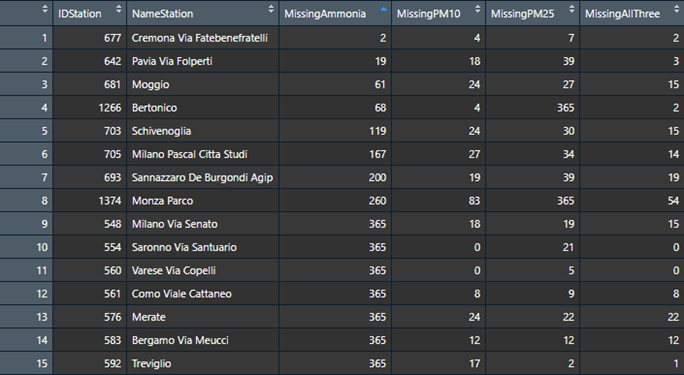
\includegraphics[scale=0.75]{Picture/b.png}
  \centering
  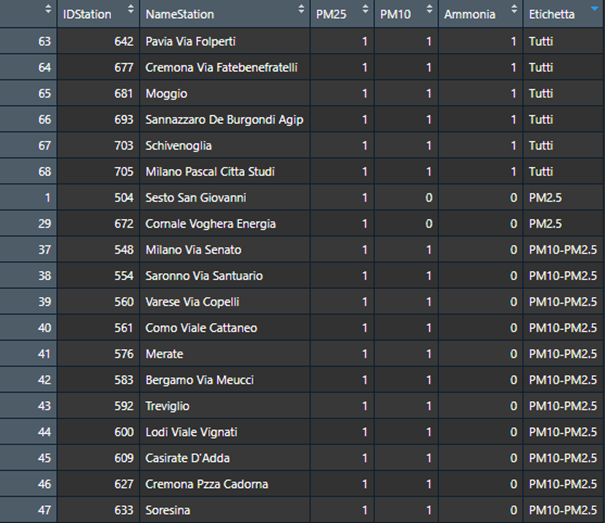
\includegraphics[scale=0.65]{Picture/PresenceTable.png}       
\end{figure}

In allegato c'è una tabella che descrive cosa viene misurato in ognuna
delle centraline prese in considerazione precedentemente (presencetableRed.csv), i dati di queste stazioni possono comunque risultare utili qualora fosse necessario un volume di dati più elevato.
\\Il risultato della mappa della Lombardia in funzione di tutte le centrali che misurano almeno uno degli inquinanti che 
vengono presi in considerazione è il seguente:

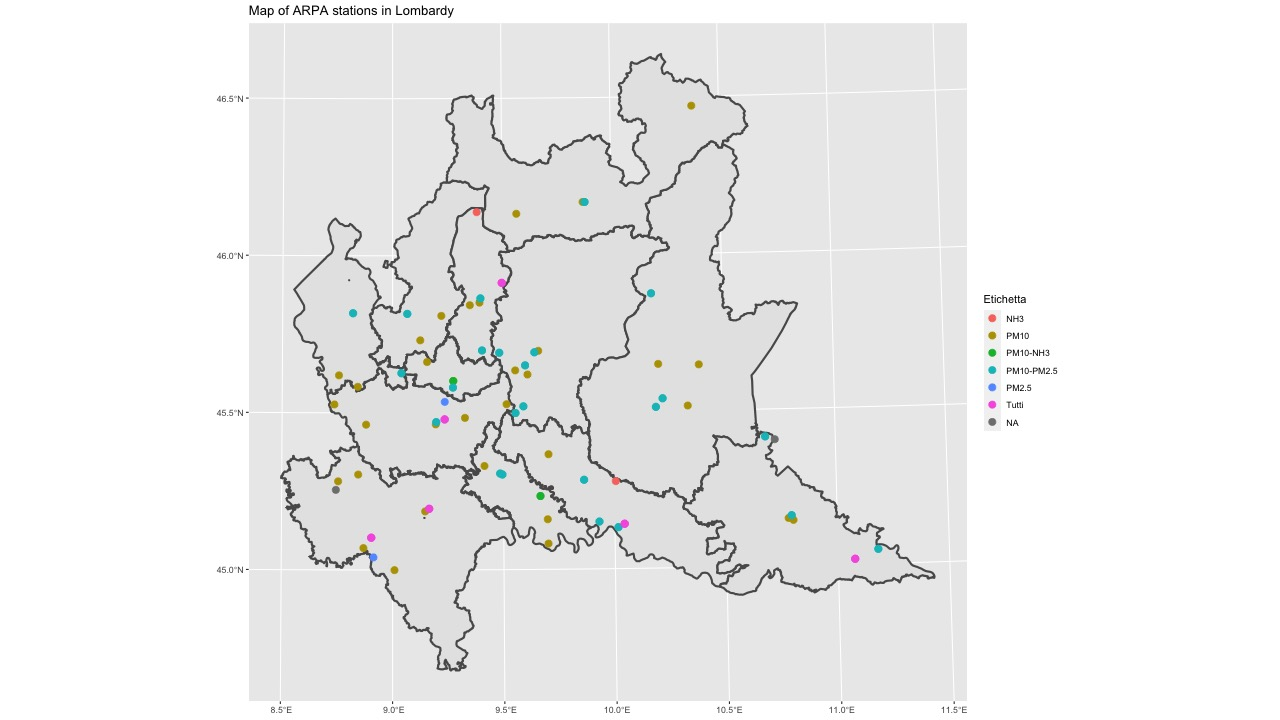
\includegraphics[scale=0.35]{Picture/mappina.jpeg}

Per ogni centralina che presenta tutti e 3 i regressori di interesse è stato fatto
un plot della serie storica, e, in presenza di un dato mancante in corrispondenza   
di uno specifico giorno, è stata tracciata una linea verticale blu.
\\La mancanza di dati può essere un fattore importante nella fase di 
costruzione del modello
e quindi sono state scelte le stazioni con il numero di missing data inferiore.
Ecco un esempio di una  delle 6 migliori centraline con un numero accettabile di dati mancanti e una con
un numero molto alto di dati mancanti (sempre appartenente alla lista delle 6 migliori centrali):

\begin{figure}[H]
    \centering
    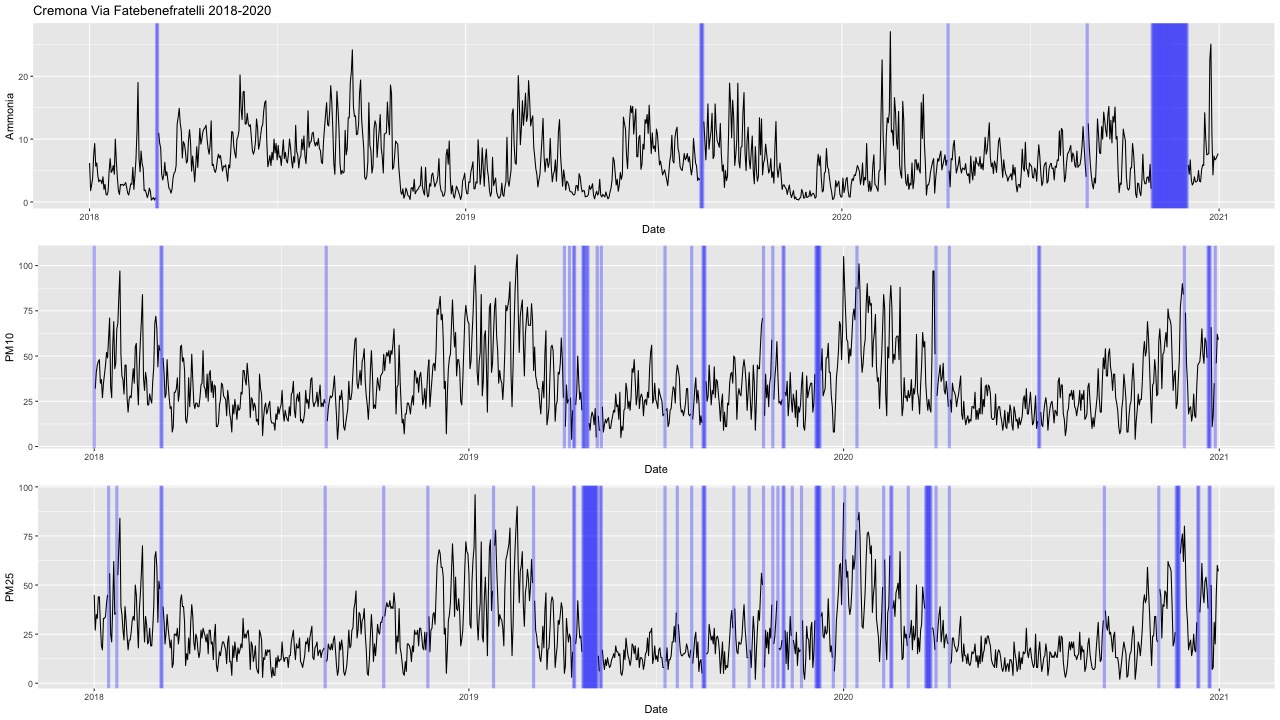
\includegraphics[scale=0.35]{Picture/Cremona Via Fatebenefratelli 2018-2020 .jpeg} 
    \caption{Cremona Via Fatebenefratelli 2018-2020, Mancanti Ammonia: 2, PM10: 4, PM25: 7, tutti e 3 contemporaneamente: 2}
    \centering
\end{figure}

\begin{figure}[H]
    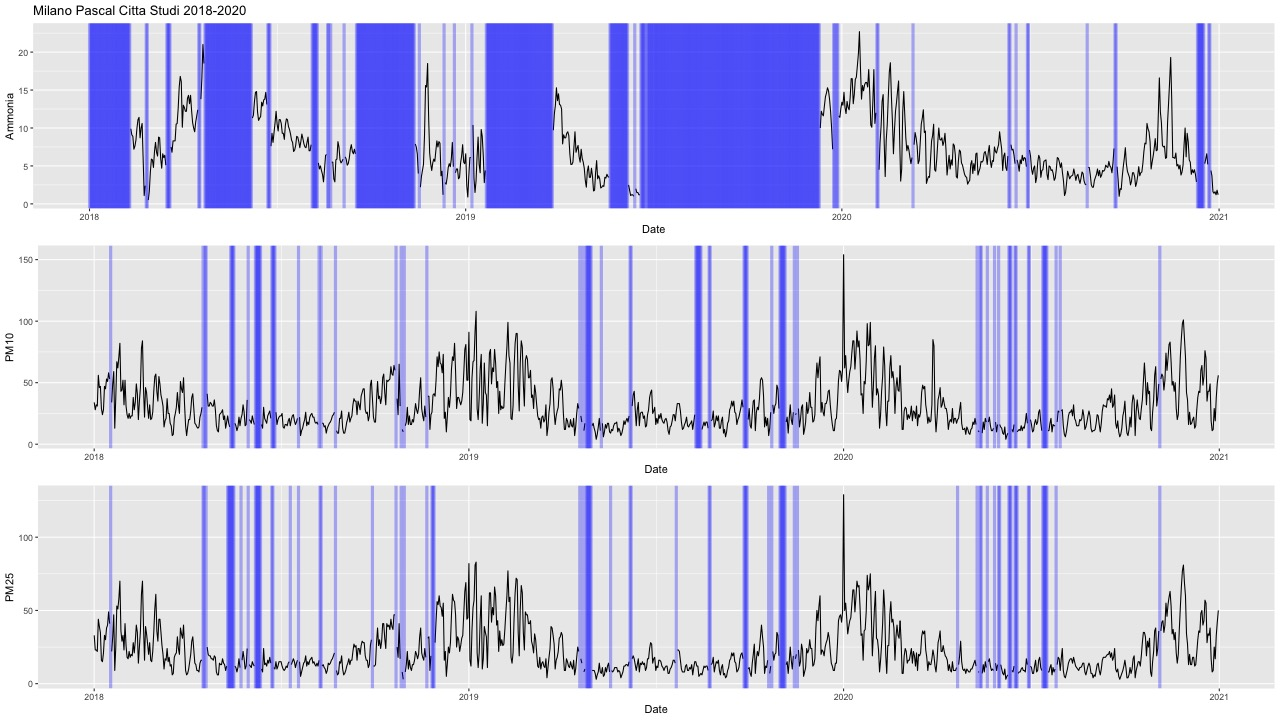
\includegraphics[scale=0.35]{Picture/Milano Pascal Citta Studi 2018-2020 .jpeg}
    \caption{Milano Pascal Citta Studi 2018-2020, Mancanti Ammonia: 167, PM10: 27, PM25: 34, tutti e 3 contemporaneamente: 14}
\end{figure}


Come si può notare da questi due grafici (ma persiste anche per tutte le altre stazioni) la variabile
più problematica, ossia quella con più dati mancanti, risulta essere l'ammoniaca.



\section{Analisi dei dati per il meteo}
Nel caso delle centraline meteorologiche, la strategia e l’obiettivo per studiare la qualità dei dati differisce da quella proposta 
per gli inquinanti. 
\\Difatti, mentre nelle variabili della qualità dell’aria l’ammoniaca e il particolato erano, 
per così dire, i bersagli, le variabili meteorologiche hanno un ruolo meramente ausiliario. 
Dopotutto, anche se il loro ruolo può essere determinante, non sono le variabili che i modelli cercheranno di predire. 
\\Di conseguenza, è stata cercata per ogni centralina che misura gli inquinanti, le due  
stazioni meteo con la distanza inferiore che prenda in considerazione contemporaneamente velocità del vento 
(wind speed), direzione del vento (wind direction), temperatura (temperature) e precipitazioni (rainfall).
E' stata utilizzata la distanza eucliedea e non è stata utilizzata la geometria sferica in quanto per distanze ridotte come quelle in considerazione, 
fungono come una accettabile approssimazione delle vere distanze, anche se non tengono conto della curvatura della Terra.
\\Infine è stata fatto un join per unire i dati delle 6 migliori stazioni con i dati delle due
stazioni meteo più vicine (allegato come NNdata.csv). 

\section{Analisi missing data per il clima}
Anche per tutti i dati meteo è stato stampata una serie storica che rappresenta i missing data nel tempo.
\\Cassina Valsassina Moggio presenta un numero quasi nullo di dati mancanti, invece Sermide E Felonica Sp 
non misura la wind speed e la wind direction praticamente fino alla fine del del 2018.
\begin{figure}[H]
  \centering
  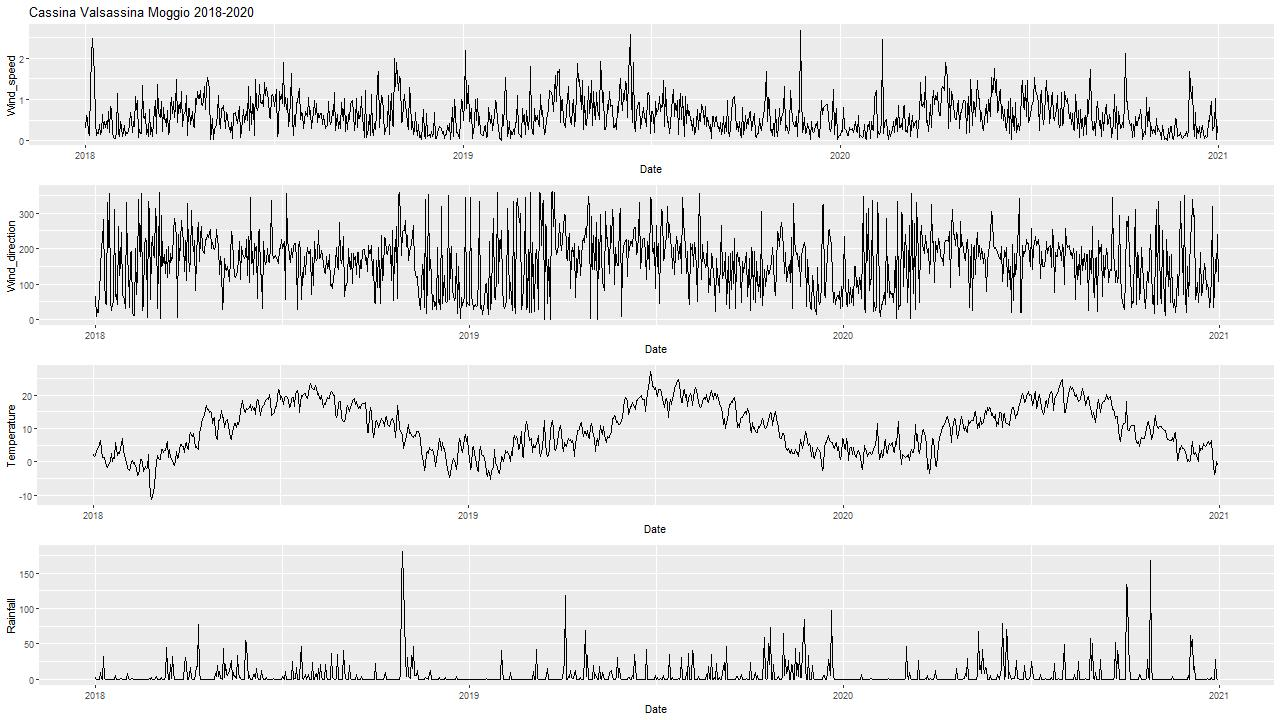
\includegraphics[scale=0.35]{Picture/Cassina Valsassina Moggio 2018-2020 .jpeg} 
  \caption{Cassina Valsassina Moggio 2018-2020}
  \centering
  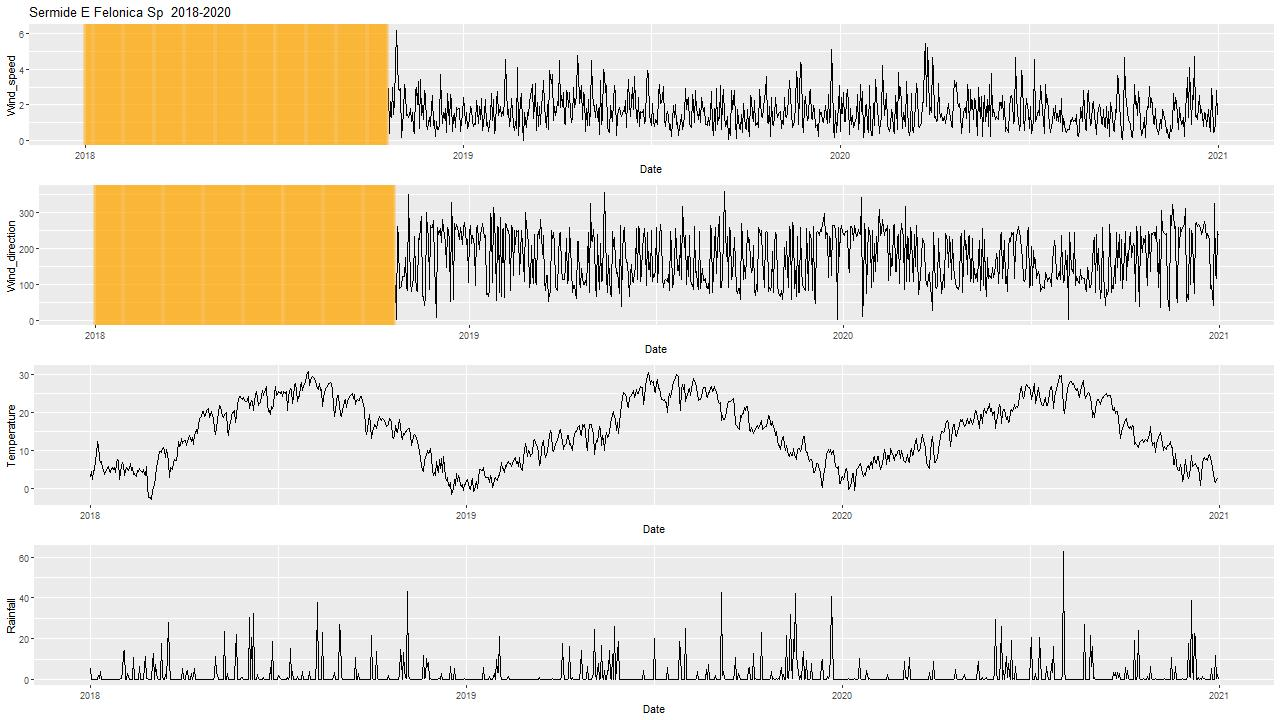
\includegraphics[scale=0.35]{Picture/Sermide.jpeg}
  \caption{Sermide E Felonica Sp  2018-2020}
\end{figure}
\end{document}
